%
% File nlp-report-isabella.tex
%
% % Based on semeval 2020 Nathan Schneider
%% Based on the style files for COLING-2020 (feiliu@cs.ucf.edu & liang.huang.sh@gmail.com), which were, in turn,
%% Based on the style files for COLING-2018, which were, in turn,
%% Based on the style files for COLING-2016, which were, in turn,
%% Based on the style files for COLING-2014, which were, in turn,
%% Based on the style files for ACL-2014, which were, in turn,
%% Based on the style files for ACL-2013, which were, in turn,
%% Based on the style files for ACL-2012, which were, in turn,
%% based on the style files for ACL-2011, which were, in turn, 
%% based on the style files for ACL-2010, which were, in turn, 
%% based on the style files for ACL-IJCNLP-2009, which were, in turn,
%% based on the style files for EACL-2009 and IJCNLP-2008...

%% Based on the style files for EACL 2006 by 
%%e.agirre@ehu.es or Sergi.Balari@uab.es
%% and that of ACL 08 by Joakim Nivre and Noah Smith

\documentclass[11pt]{article}
\usepackage{geometry}
\usepackage{coling2020}
\usepackage{times}
\usepackage{url}
\usepackage{latexsym}
\usepackage{microtype}
\usepackage{listings}
\hyphenation{an-aly-sis}
\hyphenation{an-aly-ses}
\hyphenation{Sem-Eval}
\usepackage[dvipsnames]{xcolor}
\usepackage{hyperref}
\hypersetup{
    colorlinks=true,
    linkcolor=Emerald,
    filecolor=magenta,
    urlcolor=blue,
    citecolor=RoyalBlue
}
\usepackage{graphicx}
\usepackage{textcomp}
\usepackage{outlines}
\usepackage{tabularx}
\graphicspath{ {./images/} }
\setlength\titlebox{5cm}
\colingfinalcopy

\title{SemEval-2020 Task 1: Dialogue and Narrative Coursework Report}
\author{Isabella Degen \\ University of Bristol \\ {\tt isabella.degen@bristol.ac.uk}}
\date{}

\begin{document}
    \maketitle

    \begin{abstract}
        This reports describes an embeddings based approach for finding the
        grounding documents to a user question to solve subtask 1 of the
        \href{https://doc2dial.github.io/workshop2021/shared.html}{DialDoc21 shared task}.
    \end{abstract}


    \section{Introduction}\label{sec:introduction}
    This report describes the method, experiment setup, results and conclusions for the 2021 Dialogue and Narrative
    coursework.

    The aim of this coursework was to gain more experience and to apply some of the NLP techniques we've learned during
    the semester. I focused on designing, implementing and evaluating a simple embeddings based solution for
    subtask 1 from the DialDoc21
    competition \cite{feng-etal-2020-doc2dial}.
    This allowed me to learn how such a solution compares to the submissions that topped the leaderboard,
    while developing my Python programing skills and
    learning how to implement, evaluate and keep track of experiments and results for an NLP system.

    I started off building my understanding about the Doc2Dial dataset \cite{feng-etal-2020-doc2dial} using Jupyter notebooks
    before experimenting with an embeddings algorithm called Doc2Vec from Gensim \cite{doc2vec}.
    To run multiple experiments and learn how the different hyper parameters of the Doc2Vec impacted the performance of the
    system,
    I moved the Python code into a Python module, wrote Unit Tests for the important functions, moved the configuration
    into a configuration cataclass and logged each experiment using
    the Weights \& Biases platform \cite{wandb} (For the rest of this report I'm going to refer to the Weights \& Biases
    as wandb).

    Section \ref{sec:method}
    describes the method used for each of the main steps: Understanding the data, random guessing as baseline, Doc2Vec embeddings
    and parameter experimentation. The Experiment Setup section \ref{sec:experiment-setup} and the Results section \ref{sec:results}
    keep referring back to these steps too. Finally I summarise my conclusions in \ref{sec:conclusions}


    \section{Method}\label{sec:method}

    \subsection{Understanding the Data}\label{subsec:understanding-the-data-method}
    Before starting to develop an algorithm I wanted to get an understanding of the dat available.
    There are three datasets for the Doc2dial competition available on \href{https://huggingface.co/datasets/doc2dial}{Hugging Face}:
    \begin{itemize}
        \item dialogue\_domain with data split train and validation
        \item document\_domain with data split train
        \item doc2dial\_rc with data split train and validation
    \end{itemize}

    I wanted to answer the following questions:
    \begin{itemize}
        \item What are the different datasets and how can I use them?
        \item How many grounding documents where there?
        \item How were they used in the dialogue?, How do I know which document was referenced in the dialogue?
        \item What was the format and type of the data?, What data type was the data?,
        Was the document already split into spans and how?
        \item How much data do I have?. How many spans does a document have?, How often is each span used in the dialogue?,
        Was each document used?
        \item How do I best interact and query the dataset?,Do I continue to use panda's dataframe or do I directly query
        the arrow dataset?
    \end{itemize}

    \subsection{Random Guessing as Baseline}\label{subsec:random-guessing-method}
    Before diving into an NLP algorithm solution to subtask1, I wanted gain an idea of how well a program that randomly guessed a
    grounding span scores. This served me as baseline for the rest of the work.

    \subsection{Doc2Vec embeddings}\label{subsec:doc2vc-method}
    Next I wanted to establish how well I could predict the right span of the grounding document for a user question using
    embeddings. Instead of the \texttt{word2vec} algorithm from gensim that we've used in the semester I decided to use
    \texttt{doc2vec} \cite{doc2vec} for the simple reason that I was trying to predict the most similar span to a user utterance, not jsut
    the most similar word. Doc2Vec creates a vector representation for the a document irrespective of it's length.
    While Word2Vec crates a vector for each word in the corpus, Doc2Vec creates a vector for each document in the corpus.
    In the case of subtask1 the corpus would be the grounding document form the \texttt{documents\_domain} dataset
    and the documents would be the spans or sections of these grounding documents. Once the model is trained
    it can be used to predict the n most similar documents for a new input document. To do so the vector representation
    for the new input document is calculated. This vector is then compared to all the vectors in the model. Similarity
    is established using the cosine method and the n most similar documents used during training are returned for the prediction.
    Care has to be taken to preprocess the input vectors during predictions
    the same way as the documents were processed during training.

    I trained a Doc2vec model for each of the grounding documents. This meant that I could simply predict
    the most similar span to a question using the model for that grounding document. I also trained Doc2Vec on sections instead
    of spans.

    \subsection{Parameter Experimentation}\label{subsec:experimentation-method}
    I started off implementing Doc2Vec in Jupyter notebooks and got the first initial findings. However, there are loads
    of possible configurations such as: using spans or sections as documents, different methods of preprocessing the spans, different
    hyperparameter configurations for Doc2Vec and different possibilities of creating the answers from just the most similar
    document to combining a few most similar documents. It's no wonder that I soon got lost in the Jupyter notebooks, struggled
    to remember what I've ran with which parameters and
    decided that it was time to keep track of the different experiment by moving my code into Python scripts. I also took
    the opertunity to add unit tests for the most important methods and not surprisingly found mistakes.
    Finally, I added wandb as experiment tracking platform to automatically log all configurations and results for each of
    the various runs \cite{wandb}.

    My goals was to gain a better high level understanding of what parameters affected the results for Doc2Vec and not to
    find the best Doc2Vec solution. I also wanted to learn wandb as a way to keep track of experiments and making it easier
    to reproduce experiments. As I've made the decision to train a Doc2Vec model for each grounding document and
    due to the model only being trained on the \texttt{document\_domain} dataset and not on the
    \texttt{doc2dial\_rc} dataset both the train and validation dataset of \texttt{doc2dial\_rc} could be used to validate
    the training. I ended up using 20\% of the \texttt{doc2dial\_rc} training dataset for validating the
    impact of different parameters. I varied the parameters: dm, epochs, number of most similar docs returned and weather
    the algorithm was given just the user question or also the dialogue history. To evaluate the different configurations
    I used runtime, exact match and F1 score. To evaluate the impact of different parameters I used wandb's sweep capability.


    \section{Experiment Setup}\label{sec:experiment-setup}

    All experiments were run within the nlp-2021 conda environment on my mac \cite{conda_forge_community_2015_4774216}.
    The conda environment is built and updated using the
    \href{https://github.com/isabelladegen/nlp-2021/blob/main/conda.yml}{conda.yml} file. Only the version of Python is
    fixed to 3.9, for the other libraries I wanted to use the newest version. Wandb \cite{wandb} automatically produces
    an \texttt{requirements.txt}
    file for each run that lists the exact version of each library at the time of the run to help with reproducibility. The
    \href{https://github.com/isabelladegen/nlp-2021}{Readme} on Github describes how to setup the environment as well
    as how to run a wandb experiment.

    \subsection{Understanding the Data}\label{subsec:understanding-the-data-experiment}
    I analysed the three datasets dialogue\_domain, document\_domain and doc2dial\_rc using the Jupyter Notebooks
    \href{https://github.com/isabelladegen/nlp-2021/blob/main/notebooks/DataInvestigationDoc2Dial.ipynb}{DataInvestigationDoc2Dial.ipynb}
    and \href{https://github.com/isabelladegen/nlp-2021/blob/main/notebooks/RCDataInvestigation.ipynb}{RCDataInvestigation.ipynb}.
    The notebooks download the downloaded from \href{https://huggingface.co/datasets/doc2dial}{Hugging Face}
    using \texttt{load\_datasets} and import into pandas dataframes \cite{reback2020pandas} to make use of
    \texttt{describe()}, \texttt{info()}, \texttt{value\_counts()}, \texttt{json\_normalize()}. To gain more insights
    about how the grounding documents from \texttt{document\_domain} are used in in the \texttt{dialogue\_domain},
    I wrote a procedure to combine the two and and count for each document the number of dialogs, number of turns, number of user utterances,
    number of agent utterances, number of spans, number of references to the most used span, number of spans that are never referenced.
    I also wrote a procedure to combine the \texttt{doc2dial\_rc} with \texttt{dialogue\_domain} dataset so I could understand
    this data set better. I used \texttt{matplotlib} \cite{matplotlib} and \texttt{seaborn} \cite{seaborn} to visualise
    some of my findings.

    \subsection{Random Guessing as Baseline}\label{subsec:random-guessing-experiment}
    For random guessing I loop through each of the questions in the \texttt{doc2dial\_rc} datataset and simply guess a
    random span id from the number of spans for each grounding document. The code including the results for this experiment
    can be found at the bottom of the
    \href{https://github.com/isabelladegen/nlp-2021/blob/main/notebooks/Doc2VecSolutionForSpansForSubtask1.ipynb}{Doc2VecSolutionForSpansForSubtask1.ipynb}
    Jupyter notebook. To evaluate random guessing I used the \texttt{squad\_v2} metric and built the predictions and
    references for the metric the same way the
    \href{https://github.com/doc2dial/sharedtask-dialdoc2021/blob/master/scripts/sharedtask_utils.py}{sharedtask\_utils.py}
    script does it.

    \subsection{Doc2Vec embeddings}\label{subsec:doc2vec-experiment}
    To initial Doc2Vec solution can be found in the \href{https://github.com/isabelladegen/nlp-2021/blob/main/notebooks/Doc2VecSolutionForSpansForSubtask1.ipynb}{Doc2VecSolutionForSpansForSubtask1.ipynb}
    Jupyter notebook.
    On a high level the steps are:
    \begin{outline}[enumerate]
        \1 Read the training docs for each grounding document \texttt{raw\_training\_docs\_per\_doc=\{doc\_id:[raw spans]\}}
        \1 Preprocess the docs \texttt{tokenized\_training\_docs=\{doc\_id:[\{span\_id:[tokenized and preprocessed span]\}]\}}
        \1 Train a model for each grounding document \texttt{models\_for\_doc=\{doc\_id: model\}}
        \1 Predict most similar span for each question from the \texttt{doc2dial\_rc} dataset
        \2 Preprocess the question like in step 2.
        \2 \texttt{infer\_vector()} for question
        \2 Find the most similar vector \texttt{model.dv.most\_similar([vector], topn=1)}
        \2 Find the original span for the most similar vector
        \1 Evaluate using \texttt{squad\_v2} \cite{squad2git,gitTheStandfordQADataset,Rajpurkar2016SQuAD10}
    \end{outline}

    The \href{https://github.com/isabelladegen/nlp-2021/blob/main/notebooks/Doc2VecSolutionForSectionsForSubtask1.ipynb}{Doc2VecSolutionForSectionsForSubtask1.ipynb}
    Jupyter notebook has a solution where sections are used instead of spans.

    \subsection{Parameter Experimentation}\label{subsec:experimentation-experiment}
    The python code for running the different experiments can be found in the \href{https://github.com/isabelladegen/nlp-2021/tree/main/src}{src}
    folder. There are a few different Python scripts and classes:
    \begin{outline}
        \1 \textbf{Preprocessing}: The \texttt{preprocessing\_documents.py} script loads the document domain data and creates the
        \texttt{GroundingDocument} class used by the model. The \texttt{preprocessing\_rc.py} script loads the doc2dial rc
        domain data and preprocesses the questions.
        \1 \textbf{Training \& Prediction}: The \texttt{train\_and\_predict.py} has a \texttt{TrainedModel} class that is a wrapper around
        Doc2Vec and a \texttt{BatchTrainer} that manages the models for each document.
        \1 \textbf{Evaluation}: The \texttt{evaluate.py} file is dealing with creating and running the \texttt{squad\_v2} metrics for the predictions
        \1 \textbf{Configuration}: The \texttt{Configuration.py} dataclass is used to store all the default configurations including
        the model's hyperparameters. It is also used as the \texttt{wand.config}.
        \1 \textbf{Run an experiment}: The \texttt{run\_experiment.py} script is used to run an experiment.
        The configurations used are in \texttt{configuration.py}.
        The experiment can be named and tagged here or later on the wandb website.
        \1 \textbf{Run a sweep}: The \texttt{sweep.py} script is used to run a wand sweep where multiple parameters are tested.
        There's a configuration at the top of the file that is used for the different hyper parameters to be sweeped.
        Any parameter not set there will be taken from the default configuration.
        \1 \textbf{Unit tests}: the unit tests can be found in the \href{https://github.com/isabelladegen/nlp-2021/tree/main/tests}{tests}
        folder. They have data builders to quickly create fake data and make sure everything works properly.
    \end{outline}

    Wandb automatically takes a snapshot of the Python environment, creates a requirements.txt file and uploads all this
    data to wandb. The logged the evaluation measures during the run and the hyperparameters came from the configuration
    file and got automatically logged too.

    I first ran a few experiments until I was satisfied that things were working and everything was logged correctly before
    running sweeps.


    \section{Results}\label{sec:results}

    \subsection{Understanding the Data}\label{subsec:understanding-the-data-results}

    The \textbf{\texttt{dialogue\_domain}} dataset contains all the different dialogues. The grounding document is referenced
    by \texttt{doc\_id}, the dialogue history can be found in \texttt{turns} with \texttt{utterance} being the question
    or answer by either the user or the agent marked with \texttt{role}. In \texttt{turns.references.sp\_id} the list of
    matching span ids for the grounding document is provided.

    \begin{figure}[h]
        \centering
        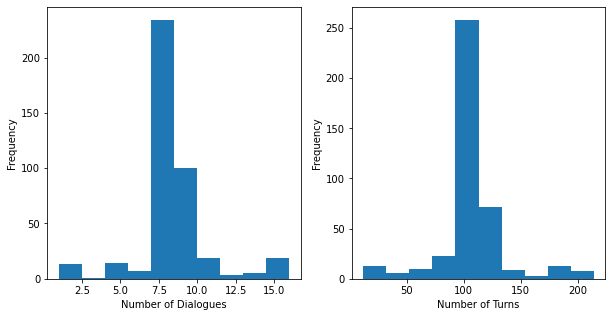
\includegraphics[width=0.8\textwidth]{number_of_dialogues_and_turns}
        \caption{Histograms for the number of dialogues per document and the number of turns per dialogue}
        \label{fig:histogram-dialogue-and-turns}
    \end{figure}

    In total there are 3474 different dialogues in the training dataset. For each document there are around eight dialogues and
    each dialogue has around a 100 turns, see figure \ref{fig:histogram-dialogue-and-turns} for teh histograms of the numbers of
    dialogues for each document and the number of turns in each dialogue.
    The training dialogue dataset only uses 415 of the 488 grounding documents.\\

    The \textbf{\texttt{document\_domain}} dataset contains all the different grounding documents. Note that this dataset does not have
    a training and validation data split and all documents used for training and validation are in the train split.
    The documents share the same \texttt{doc\_id} with the \texttt{dialogue\_domain}. The full text of the document
    can be found in \texttt{doc\_text}. The documents are already preprocessed into spans \texttt{spans} which themselves
    use the \texttt{id\_sp} that then refers back to the \texttt{sp\_id} used in the dialogue's turns. The \texttt{text\_sp}
    contains the span text.

    \begin{figure}[h]
        \centering
        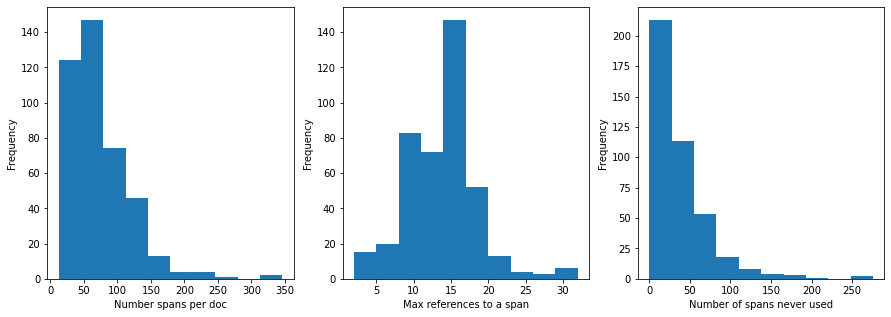
\includegraphics[width=0.8\textwidth]{span_counts}
        \caption{Histograms for the number of spans per document, the max number of references to the same span in a dialogue and the number of
        spans never referenced in a dialogue }
        \label{fig:histogram-spans}
    \end{figure}

    There are 488 different grounding documents in the dataset that come from 5 different domains. Each document has
    around 50 different spans. Some spans are referenced multiple times in a dialogue, the max number of references
    to the same span are around 16. Most documents have spans that are never used, this is usually in the tens but for a few documents
    this is significantly higher; see figure \ref{fig:histogram-spans} for the histograms.

    I also created a heat map to visualise how frequent the spans from the different documents were used in the \texttt{dialogue\_domain},
    see figure \ref{fig:heat-map-all-spans}. Given that the documents have different numbers of span, I set the frequency for spans that did not exist to -10. These
    are therefore shown as the darkest colour in the figure. Bighter colours mean that spans is referenced more frequently in a
    dialogue. I also included a figure that shows the heatmap just for the first 30 documents and their first 30 spans
    so the numbers become visible, see figure \ref{fig:heat-map-first-30-spans}. Both graphics show that most spans
    are hardly ever referenced and a few are very frequently referenced. This needs to be taken into account when
    deciding which algorithm is going to be used used to learn what's the best grounding span for a user utterance.

    \begin{figure}[h]
        \centering
        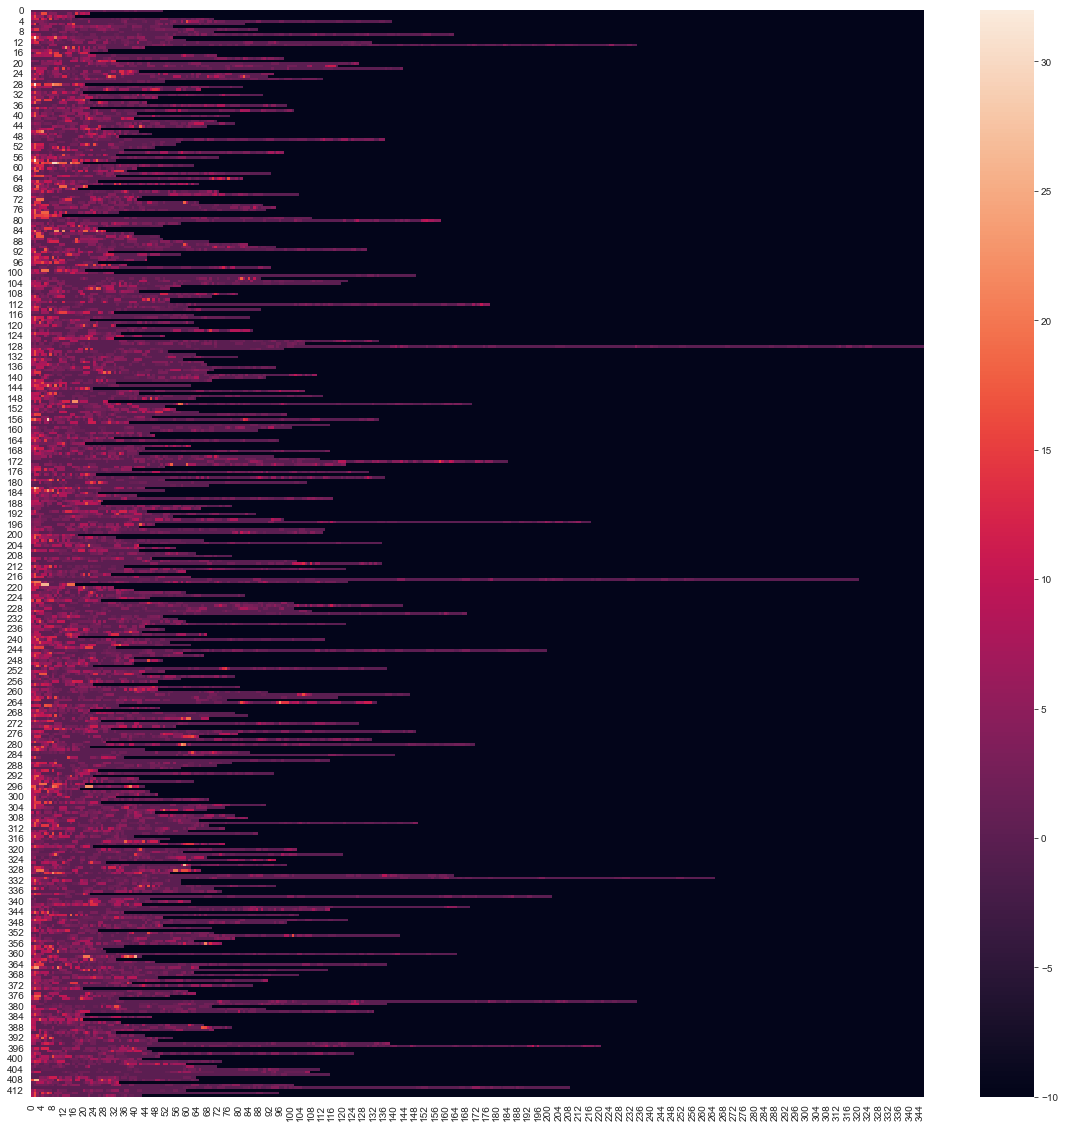
\includegraphics[width=0.8\textwidth]{sparsity_of_spans}
        \caption{Heat map of the frequency a span is referenced in a dialogue. Bright fields indicate spans that are frequently
        referenced in a dialogue, black means that span does not exist in that document}
        \label{fig:heat-map-all-spans}
    \end{figure}

    \begin{figure}[h]
        \centering
        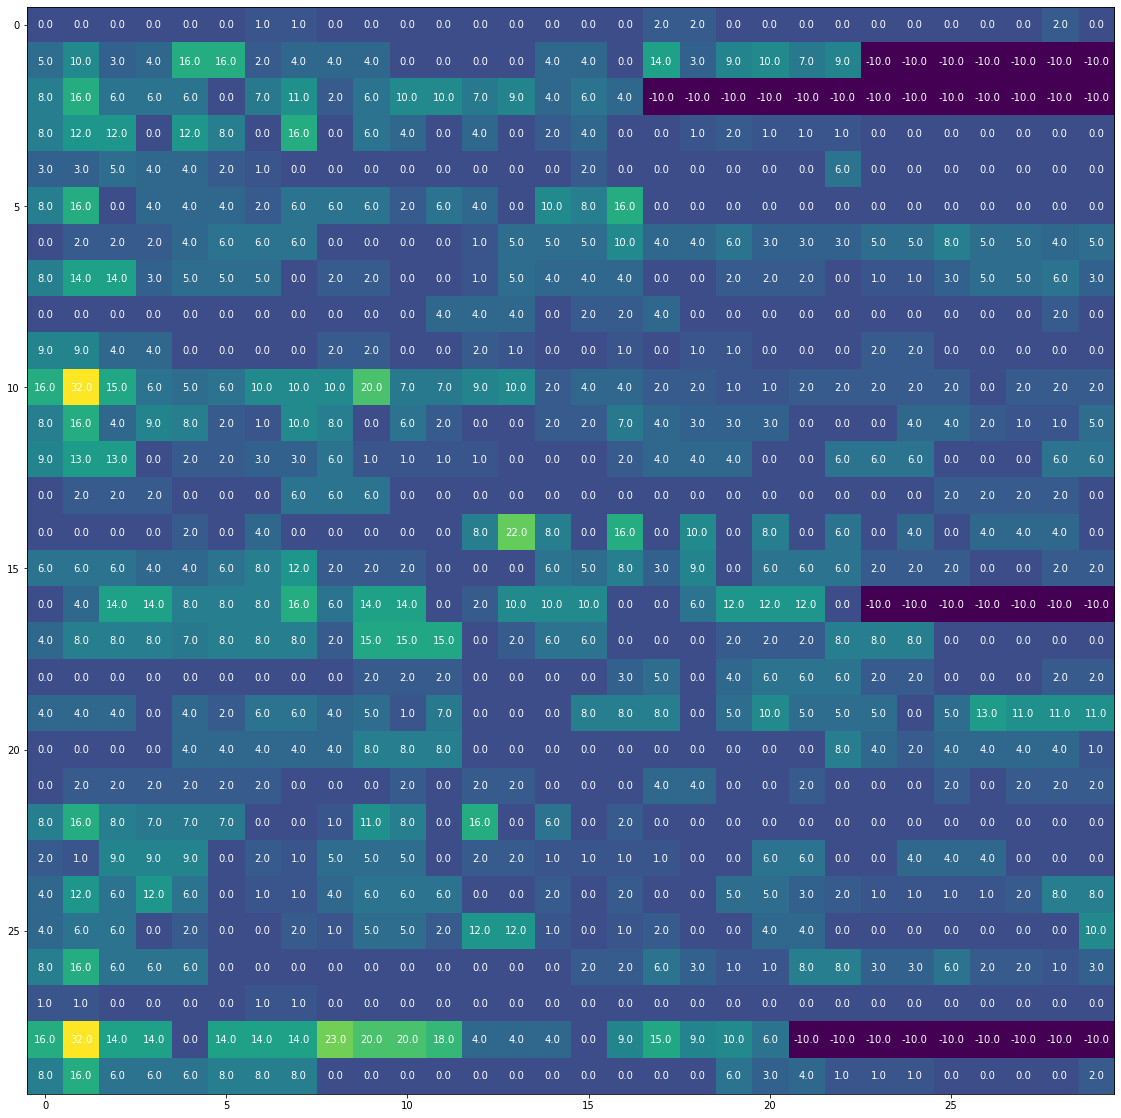
\includegraphics[width=0.8\textwidth]{sub_section_usage_of_spans}
        \caption{Heat map of the first 30 documents and the number of references to their first 30 spans. Violet or the number
        -10 indicates the span did not exist}
        \label{fig:heat-map-first-30-spans}
    \end{figure}

    Initially, I thought I needed to create a list of user utterances and the dialogue history for which I need to find the
    grounding document myself using the \texttt{turns} from the \texttt{dialogue\_domain} dataset. When investigating how
    to get the provided \href{https://github.com/doc2dial/sharedtask-dialdoc2021/blob/master/scripts/sharedtask_utils.py}{scoring script}
    to work, I learned that it was easiest to use the \textbf{\texttt{doc2dial\_rc}} dataset.
    This dataset refers to the grounding documents \texttt{doc\_id} by \texttt{title}.
    The \texttt{id} is the combination of the \texttt{dialogue\_id\_turn\_id}. \texttt{question} is the dialogue history starting
    with the the user question that the grounding document should be found for and listing the previous dialogue at each step.
    Utterances for the user are marked with a \texttt{user:}, those of the agent are marked with \texttt{agent:}. Not
    all user utterances have their own \texttt{doc2dial\_rc} data row. User's comments or confirmations, e.g \textit{Yes.} and
    \textit{Ok.} are omitted.

    \subsection{Random Guessing as Baseline}\label{subsec:random-guessing-results}

    Random guessing of the 20431 question in the \texttt{doc2dial\_rc} training dataset achieved an F1 score of 11.73
    and an exact match of 1.14. For the 3972 questions in the validation dataset the F1 score was 15.37 and the exact match
    was 1.26. These numbers obviously vary for each run but stay within the range.

    \subsection{Doc2Vec embeddings}\label{subsec:doc2vec-results}

    The initial results for Doc2Vec and in its default configuration and using their preprocessing method is shown
    in table \ref{table:simple-doc2vec-results}. Unsurprisingly the results are not fantastic but better than random
    guessing. I should have also done random guessing for sections to do a proper analysis of sections vs spans.

    \begin{table}[h!]
        \centering
        \begin{tabular}{|l|l|l|l|}
            \hline
            Metrics     & Doc2Vec Spans & Doc2Vec Sections & Random Guessing Spans \\ \hline
            F1 Score    & 15.26         & 17.26            & 11.73                 \\ \hline
            Exact Match & 1.43          & 0.85             & 1.14                  \\ \hline
        \end{tabular}
        \caption{Doc2Vec for spans and sections compared to random guessing for spans}
        \label{table:simple-doc2vec-results}
    \end{table}

    \subsection{Parameter Experimentation}\label{subsec:experimentation-results}

    Table \ref{table:simple-doc2vec-results} explains the different parameters configurations and how they influence
    the F1 score and exact match. Parameters that do well for F1 seem to effect exact match negatively and
    visa versa. Good parameters for F1 are dm 0 (Bag of words), using 150 epochs, not using the history of the question
    and using the two or three most likely spans for the answer. Bigger vector sizes work better but it's not as
    important as the other parameters, see table \ref{table:5-best-f1}. Bad parameters for F1 are only using the on most likely span to answer,
    keeping the dialogue history, using only 50 epochs, dm 1. Smaller vector sizes tend to result in less good F1 scores
    but again it's not as influential as the other parameters, see table \ref{table:5-worst-f1}. On the other hand good parameters for exact match are
    only using the most likely span (direct contradiction to F1), not using the dialogue history,
    using more than 100 epochs and generally bigger vector sizes work better but again it's not as influential, see table
    \ref{table:5-best-exact}. Bad parameters
    for exact match are, using the three most likely spans, see table \ref{table:5-worst-exact}.
    The other parameters matter too but are not as important for exact match. Unsurprisingly the best parameters for runtime are,
    dm 0, using few epochs and smaller vector sizes, see table \ref{table:5-best-runtime}. However these lead to worse F1 and exact match. However, the
    runtime was not a limiting factor with Doc2Vec in the setup that I've used it.

    The parallel coordinates chart also show the impact of different parameters on the F1 score and
    exact match, see figures \ref{fig:parallel-coordinates-f1} and \ref{fig:parallel-coordinates-exact-match}.

    \begin{figure}[h]
        \centering
        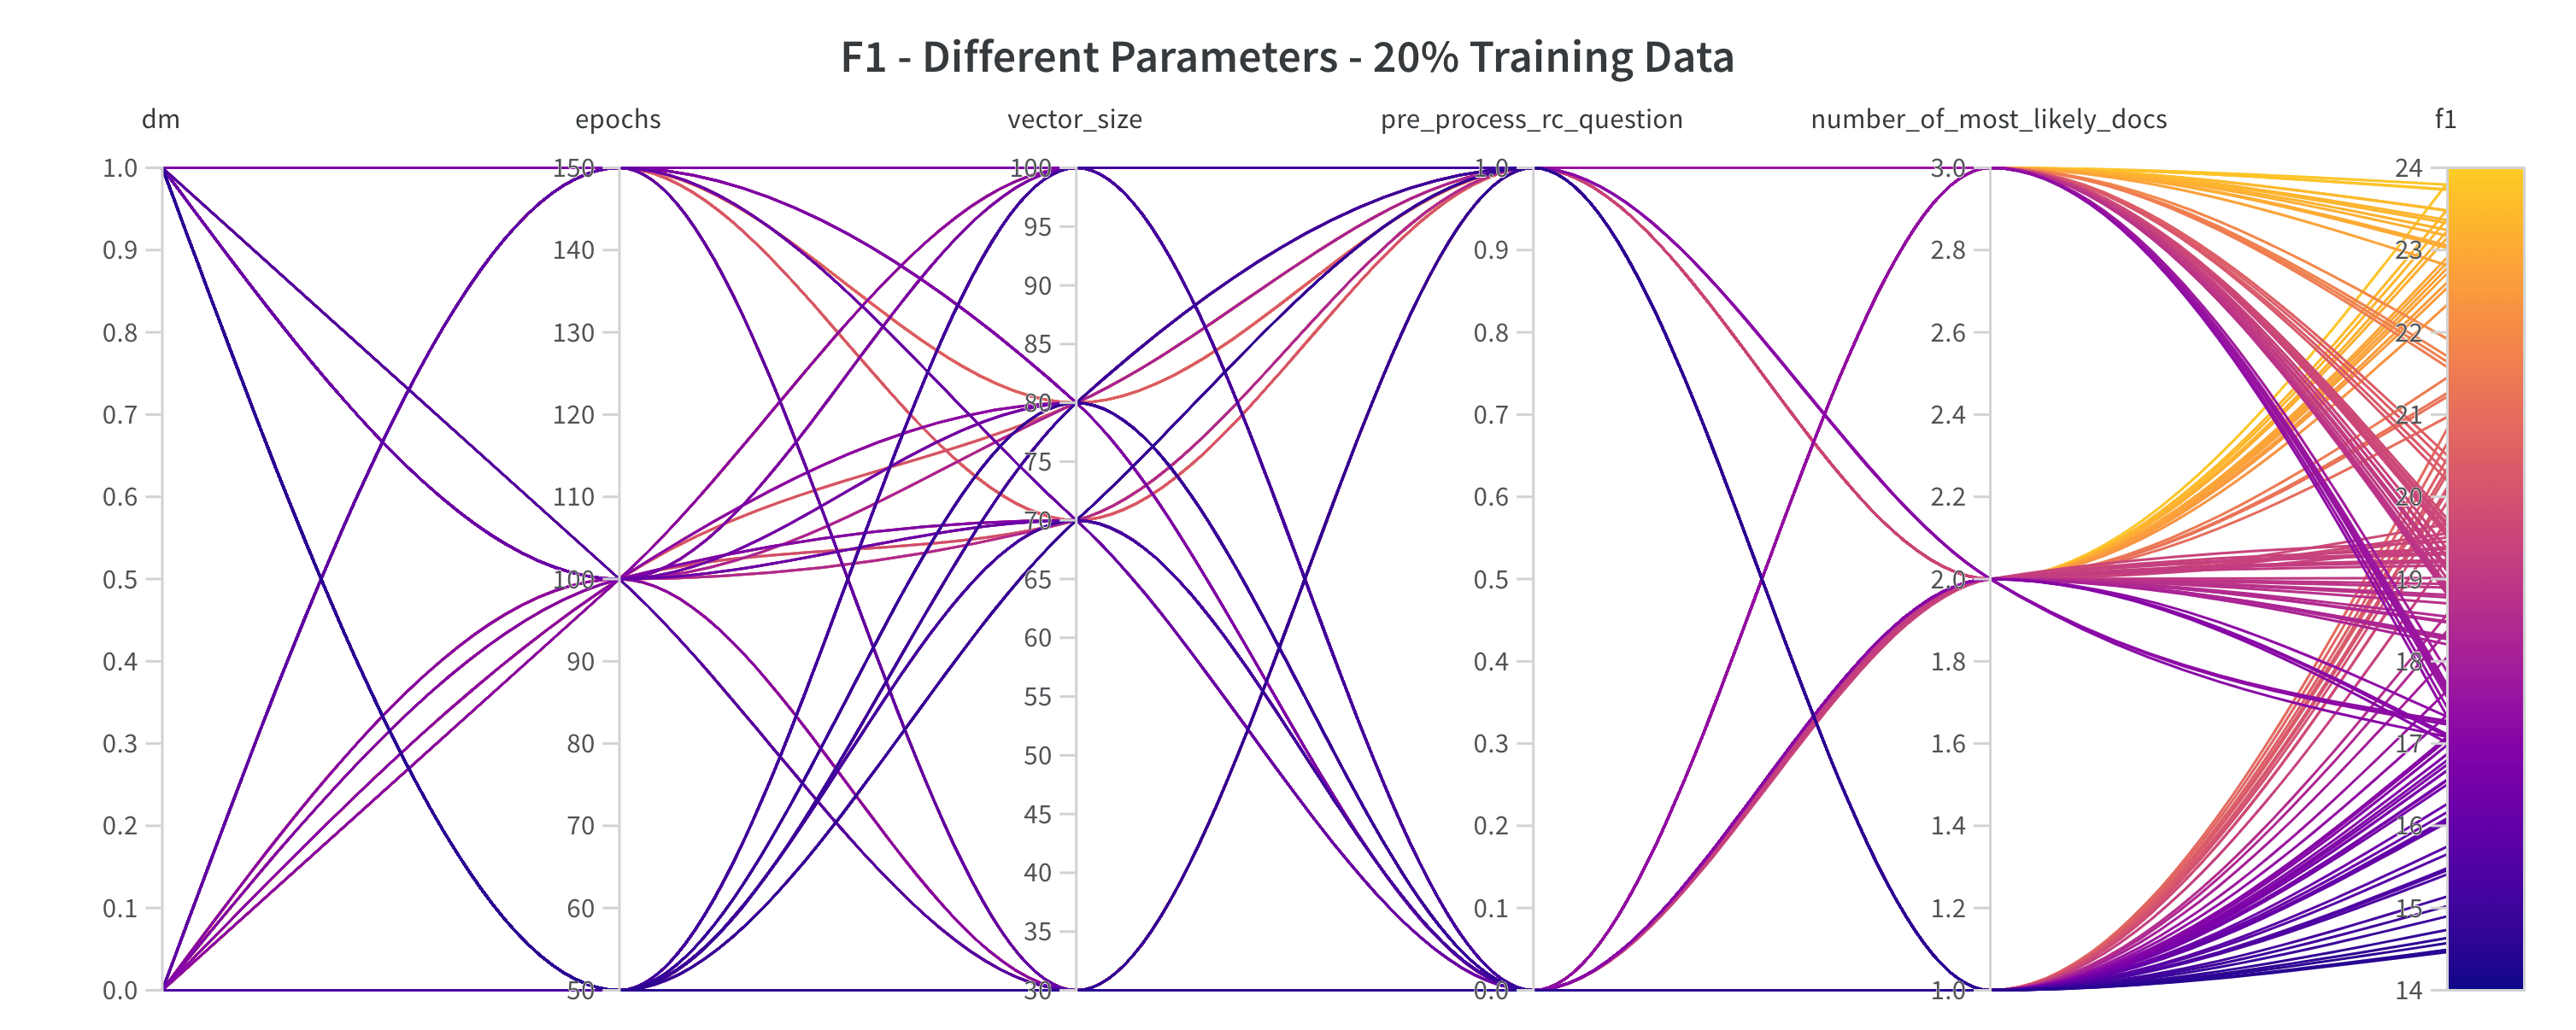
\includegraphics[width=0.8\textwidth]{parallel-coordinates-F1}
        \caption{Parallel coordinates chart for F1 score}
        \label{fig:parallel-coordinates-f1}
    \end{figure}

    \begin{figure}[h]
        \centering
        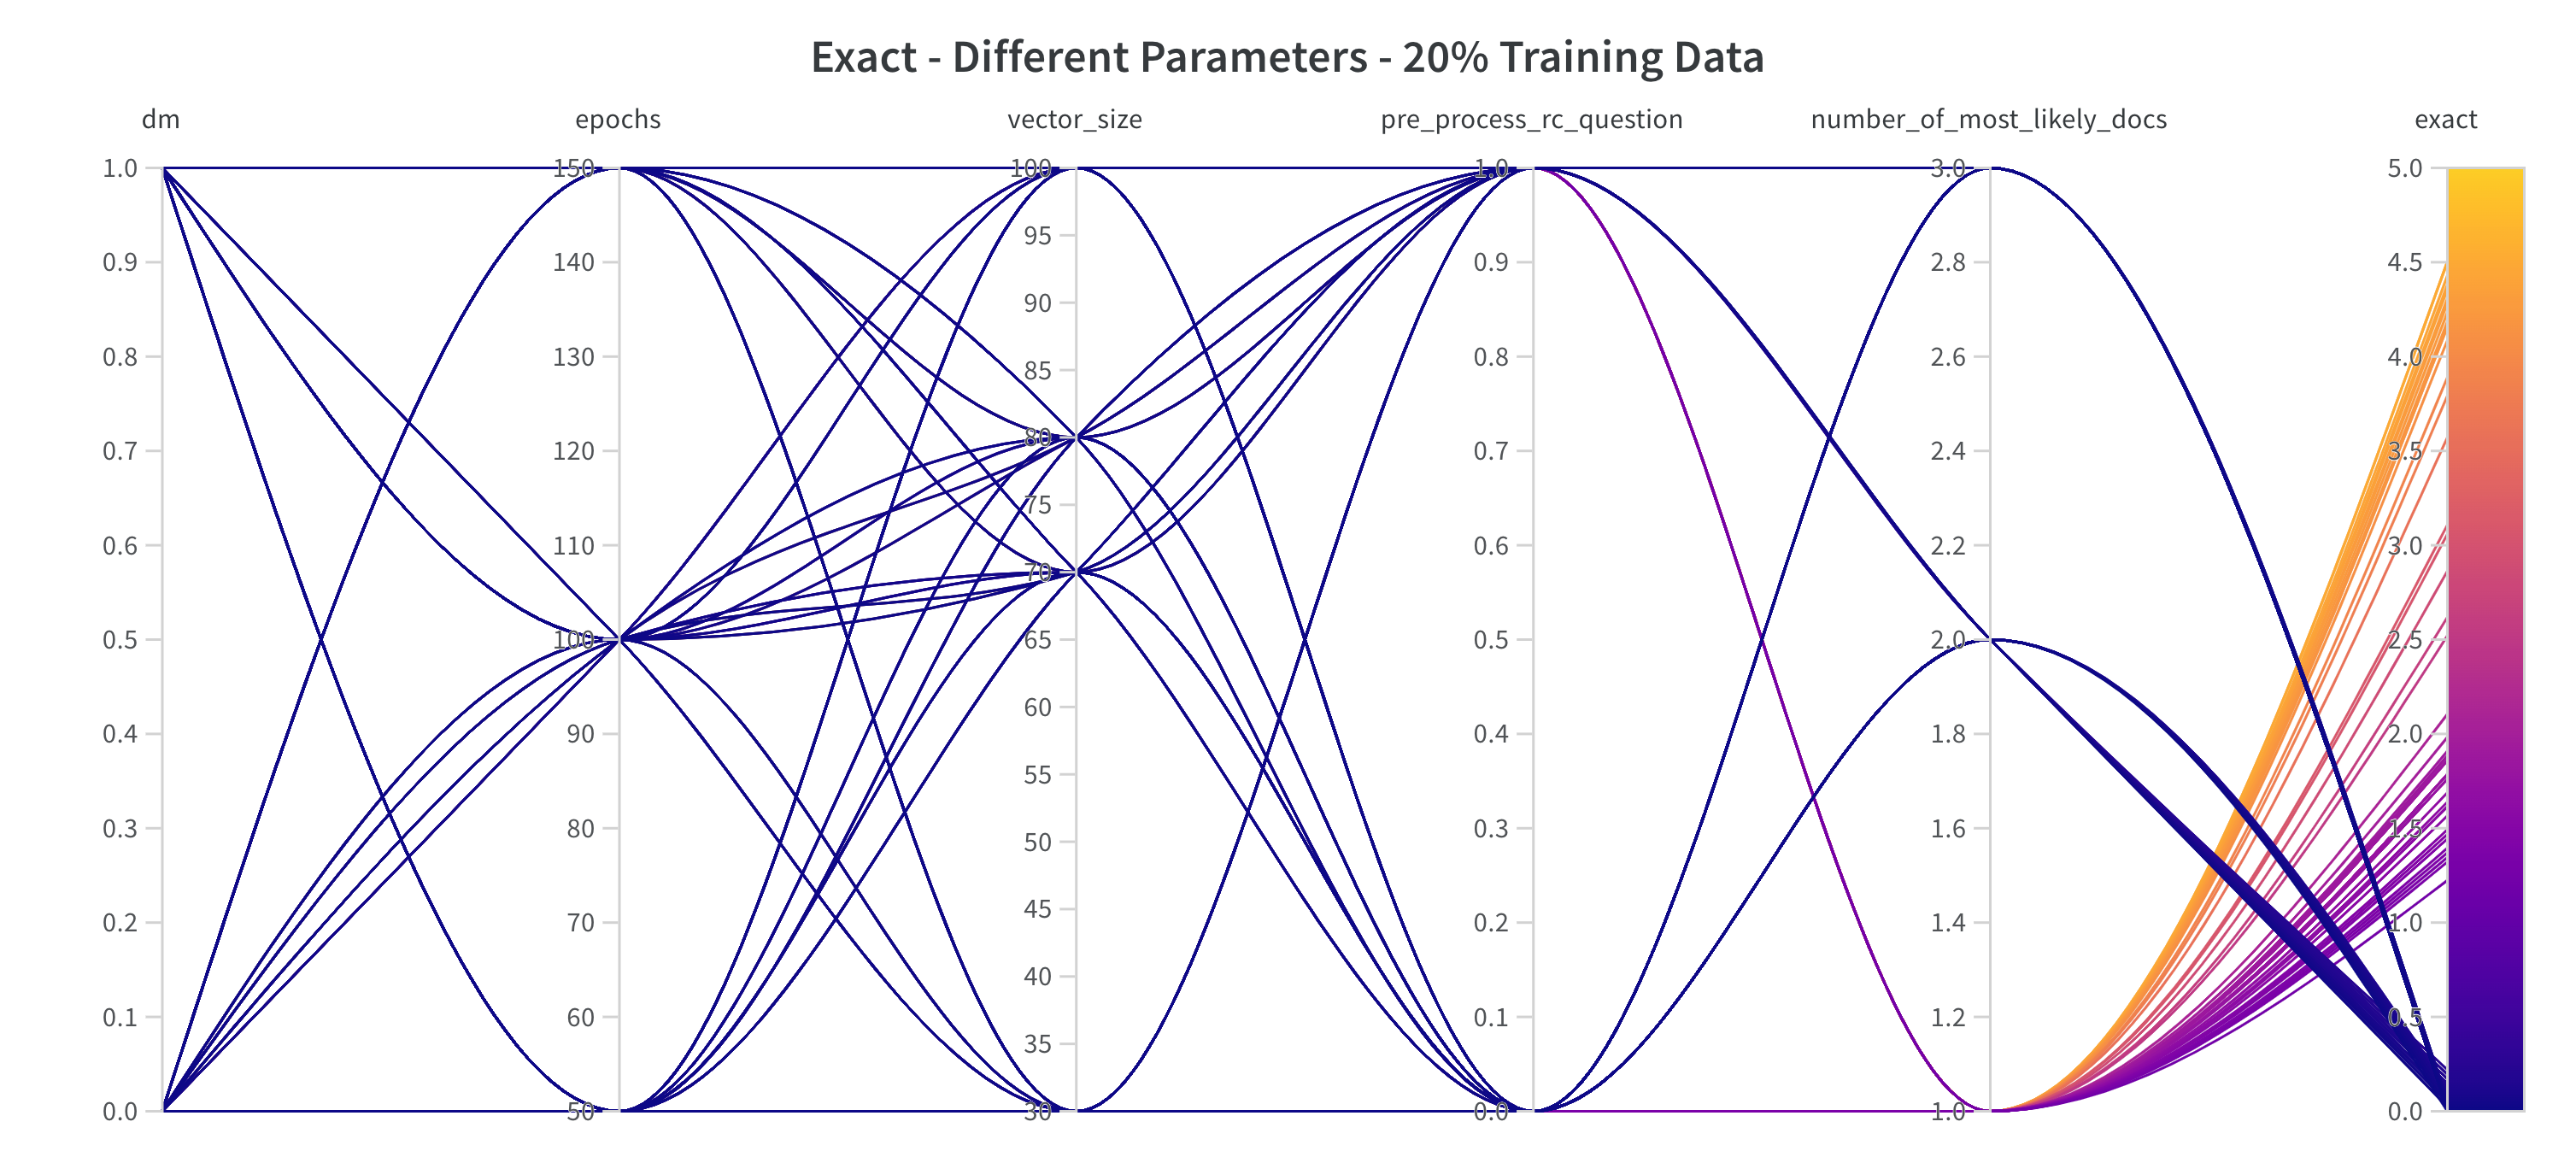
\includegraphics[width=0.8\textwidth]{parallel-coordinates-exact-match}
        \caption{Parallel coordinates chart for exact match}
        \label{fig:parallel-coordinates-exact-match}
    \end{figure}


    \section{Conclusions}\label{sec:conclusions}

    My solution is not surprisingly inferior to the submissions that topped the leaderboard. However, after a little bit
    of tuning it achieved F1 scores of around 23 and was better than random guessing a span from the grounding document.
    F1 and exact match are hard to both optimise: a better F1 in my experiment directly lead to worse exact match.
    To achieve a good exact match
    only the most likely span should be used. This has to do with the the model returning spans even when they are not next to
    each other in the document. However, for utterances that have more than one grounding span,
    these grounding spans follow each other and are not from all over the document. I can think of two ways to improve this:
    return more than one most likely
    span but only if they are next to each other, use sections instead of spans as this showed to be more promising.
    However, I've not tried these. Table \ref{table:simple-doc2vec-results} summarieses a few conclusions about the
    different hyper parameters.

    I've certainly learned a lot and became more familiar with how to implement an NLP system. Based on this experience I would do a
    few things differently:
    \begin{itemize}
        \item Focusing first on building the simplest system end to end before diving into data analysis. I spent a lot of
        time analysing the dialogue dataset that I didn't even ended up using. I believe having the system working end to
        end provides a good focus on what areas need analysing.
        \item Writing pure Python using test-driven development from the beginning. I had quite a few bad bugs in my
        Jupyter notebook code that I would have found earlier. The tests, when written well, can also be a great living
        document on how the code works.
        \item Use an experiment tracking tool and keep all configuration away from the rest of the code from the get go.
        I spend a lot of time forgetting what I've tried and remembering F1 scores I then never could achieve again. Using
        an experiment tracking tool certainly helped me being able to reproduce and remember what I've tried and what results
        this achieved.
        \item Be prepared to try different solutions quickly and setting up a pipeline where the model can be easily changed
        to many different models.
    \end{itemize}

    I've already made use of these learning for my other coursework.

    \bibliographystyle{coling}
    \bibliography{bibliography}

    \begin{table}[p]
        \centering
        \begin{tabularx}{\textwidth}{|X|X|X|X|X|X|X|X|X|}
            \hline
            Sweep no & Runtime (s) & Vector Size & Dm & Epochs & Pre process Question & \# Most Likely Spans & F1 & Exact Match \\ \hline
            64       & 59          & 100         & 0  & 150    & 1                    & 2                    & 23.82 & 0.15        \\ \hline
            72       & 61          & 100         & 0  & 150    & 1                    & 3                    & 23.80 & 0.02        \\ \hline
            70       & 61          & 70          & 0  & 150    & 1                    & 3                    & 23.74 & 0.02        \\ \hline
            71       & 58          & 80          & 0  & 150    & 1                    & 3                    & 23.73 & 0.02        \\ \hline
            63       & 58          & 80          & 0  & 150    & 1                    & 2                    & 23.49 & 0.12        \\ \hline
        \end{tabularx}
        \caption{5 best configurations for F1 score}
        \label{table:5-best-f1}
    \end{table}

    \begin{table}[p]
        \centering
        \begin{tabularx}{\textwidth}{|X|X|X|X|X|X|X|X|X|}
            \hline
            Sweep no & Runtime (s) & Vector Size & Dm & Epochs & Pre process Question & \# Most Likely Spans & F1 & Exact Match \\ \hline
            1        & 41          & 30          & 0  & 50     & 0                    & 1                    & 15.46 & 1.49        \\ \hline
            97       & 86          & 30          & 1  & 100    & 0                    & 1                    & 15.41 & 1.47        \\ \hline
            80       & 41          & 100         & 1  & 50     & 1                    & 1                    & 15.14 & 1.64        \\ \hline
            74       & 51          & 70          & 1  & 50     & 0                    & 1                    & 15.02 & 1.62        \\ \hline
            76       & 53          & 100         & 1  & 50     & 0                    & 1                    & 14.90 & 1.40        \\ \hline
        \end{tabularx}
        \caption{5 worst configurations for F1 score}
        \label{table:5-worst-f1}
    \end{table}

    \begin{table}[p]
        \centering
        \begin{tabularx}{\textwidth}{|X|X|X|X|X|X|X|X|X|}
            \hline
            Sweep no & Runtime (s) & Vector Size & Dm & Epochs & Pre process Question & \# Most Likely Spans & F1 & Exact Match \\ \hline
            56       & 60          & 100         & 0  & 150    & 1                    & 1                    & 20.83 & 4.50        \\ \hline
            30       & 46          & 70          & 0  & 100    & 1                    & 1                    & 19.72 & 4.50        \\ \hline
            54       & 59          & 70          & 0  & 150    & 1                    & 1                    & 20.47 & 4.43        \\ \hline
            127      & 94          & 80          & 1  & 150    & 1                    & 1                    & 20.28 & 4.38        \\ \hline
            55       & 59          & 80          & 0  & 150    & 1                    & 1                    & 20.66 & 4.36        \\ \hline
        \end{tabularx}
        \caption{5 best configurations for exact match}
        \label{table:5-best-exact}
    \end{table}

    \begin{table}[p]
        \centering
        \begin{tabularx}{\textwidth}{|X|X|X|X|X|X|X|X|X|}
            \hline
            Sweep no & Runtime (s) & Vector Size & Dm & Epochs & Preprocess Question & \# Most Likely Spans & F1 & Exact Match \\ \hline
            113      & 86          & 30          & 1  & 100    & 0                   & 3                    & 19.00 & 0           \\ \hline
            140      & 144         & 100         & 1  & 150    & 0                   & 3                    & 19.55 & 0           \\ \hline
            24       & 30          & 100         & 0  & 50     & 1                   & 3                    & 20.19 & 0           \\ \hline
            17       & 38          & 30          & 0  & 50     & 0                   & 3                    & 19.10 & 0           \\ \hline
            21       & 30          & 30          & 0  & 50     & 1                   & 3                    & 20.50 & 0           \\ \hline
        \end{tabularx}
        \caption{5 worst configurations for exact match}
        \label{table:5-worst-exact}
    \end{table}

    \begin{table}[p]
        \centering
        \begin{tabularx}{\textwidth}{|X|X|X|X|X|X|X|X|X|}
            \hline
            Sweep no & Runtime (s) & Vector Size & Dm & Epochs & Preprocess Question & \# Most Likely Spans & F1 & Exact Match \\ \hline
            15       & 29          & 80          & 0  & 50     & 1                   & 2                    & 19.56 & 0.17        \\ \hline
            23       & 30          & 80          & 0  & 50     & 1                   & 3                    & 20.40 & 0           \\ \hline
            22       & 30          & 70          & 0  & 50     & 1                   & 3                    & 20.28 & 0           \\ \hline
            24       & 30          & 100         & 0  & 50     & 1                   & 3                    & 20.19 & 0           \\ \hline
            21       & 30          & 30          & 0  & 50     & 1                   & 3                    & 20.50 & 0           \\ \hline
        \end{tabularx}
        \caption{5 best configurations for runtime including preprocessing, training and prediction time}
        \label{table:5-best-runtime}
    \end{table}

    \begin{table}[p]
        \centering
        \begin{tabularx}{\textwidth}{|X|X|X|X|X|X|X|X|X|}
            \hline
            Sweep no & Runtime (s) & Vector Size & Dm & Epochs & Preprocess Question & \# Most Likely Spans & F1 & Exact Match \\ \hline
            122      & 125         & 70          & 1  & 150    & 0                   & 1                    & 16.87 & 1.86        \\ \hline
            141      & 127         & 30          & 1  & 150    & 1                   & 3                    & 23.18 & 0           \\ \hline
            138      & 127         & 70          & 1  & 150    & 0                   & 3                    & 19.12 & 0.02        \\ \hline
            124      & 127         & 100         & 1  & 150    & 0                   & 1                    & 17.05 & 1.86        \\ \hline
            129      & 128         & 30          & 1  & 150    & 0                   & 2                    & 18.78 & 0.05        \\ \hline
        \end{tabularx}
        \caption{5 worst configurations for runtime including preprocessing, training and prediction time}
        \label{table:5-worst-runtime}
    \end{table}

    \begin{table}[p]
        \centering
        \begin{tabularx}{\textwidth} {|X|X|X|X|X|}
            \hline
            \textbf{Parameter} &
            \textbf{Range} &
            \textbf{F1} &
            \textbf{Exact match} &
            \textbf{Summary} \\ \hline
            \textbf{Vector size} &
            30, 70, 80, 100 &
            \textgreater{}30 works well &
            \textgreater{}30 works well &
            Surprisingly, not that influential as long as it's not too small \\ \hline
            \textbf{DM} &
            0: PV-DBOW, bag of words; 1: PV-DM, distributed memory &
            PV-DBOW works better &
            PV-DBOW works better &
            Surprisingly, it works better to treat each span as a bag of words instead of attempting to learn places of words within a span \\ \hline
            \textbf{Epochs} &
            50, 100, 150 &
            More work better &
            More work better &
            Unsurprisingly, more epochs work better, but they also mean a significant increase in training time \\ \hline
            \textbf{Preprocess Question} &
            0: rc question including history; 1: only the first 'user:' question of each rc question → excluding the dialogue history &
            Better to just pass the question without the dialogue history &
            Clearly better to not pass the history and only pass the current question &
            Given that this model evaluates the similarity between to documents (question and spans of the grounding doc)
            it's not surprising that the history of what came before does not matter and actually hinders the performance \\ \hline
            \textbf{\# Of Most Likely Spans} &
            1, 2, 3: Number of most likely spans returned and combined into the most likely answer &
            Better to return top 3 most likely spans &
            Better to only return the most likely span. Both two and three most likely spans perform badly &
            Directly opposite influence on F1 and exact match. This might also be because the x most likely spans are not
            forced to follow each other in the document which is bad for exact match \\ \hline
        \end{tabularx}
        \caption{Overview different Doc2Vec hyperparameters impacting F1 score and exact match}
        \label{table:simple-doc2vec-results}
    \end{table}

\end{document}
